% =============================================================================
% artigo-alpha: versão preliminar do artigo (22/10/2026), só com as três testnets públicas.
%
% - Serve de base para a escrita final; o texto definitivo vai para o template do
%   COTB 2027 (paper/template_cotb2027.tex), sem mudar a formatação do template.
% - Todos os números vêm de pesquisa/3-resultados/resultados.md (npm run analisar).
%   Se a análise for refeita, atualize as tabelas daqui junto.
% - \pendente{...} marca o que falta escrever, conferir ou citar. Nenhum pode
%   sobrar na versão enviada.
% - Regras do template (matriz, seção 13): até 6 páginas com referências; título,
%   abstract e keywords em inglês; citações numéricas; versão de avaliação anônima;
%   Declaração de Uso de IA obrigatória; não identificar o banco parceiro.
%
% Compilar (dentro de artigo/): latexmk -pdf artigo-alpha.tex   (TinyTeX em ~/.TinyTeX; binários em ~/.local/bin)
% Pacote faltando: tlmgr install <pacote>
% =============================================================================
\documentclass[10pt,a4paper]{article}

\usepackage[T1]{fontenc}
\usepackage[utf8]{inputenc}
\usepackage[english,brazilian]{babel}
\usepackage{lmodern}
\usepackage[margin=2.2cm]{geometry}
\usepackage{graphicx}
\usepackage{booktabs}
\usepackage{tabularx}
\usepackage{multirow}
\usepackage{amsmath}
\usepackage{xcolor}
\usepackage{caption}
\usepackage[hidelinks]{hyperref}

\graphicspath{{../pesquisa/3-resultados/graficos/}{figuras/}}

\newcommand{\pendente}[1]{\textcolor{red}{[#1]}}
\newcommand{\fn}[1]{\texttt{#1}}

\title{Seleção de rede blockchain para crédito interfinanceiro overnight com liquidação DvP: uma avaliação multicritério em testnets públicas\\[0.6em]
\large Blockchain network selection for overnight interbank lending with DvP settlement: a multi-criteria evaluation on public testnets}
\author{\pendente{Autores omitidos na versão de avaliação}}
\date{}

\begin{document}
\maketitle

% -----------------------------------------------------------------------------
\begin{otherlanguage}{english}
\begin{abstract}
Overnight interbank lending still relies on manual limit checks and reconciliation, which delay settlement and increase counterparty risk. This paper asks which blockchain network is most suitable for running an overnight interbank lending protocol with delivery-versus-payment (DvP) settlement. We frame the choice as a multi-attribute decision problem with five criteria weighted by the Analytic Hierarchy Process (AHP): resilience under load (29.78\%), contract security (29.78\%), latency (15.78\%), cost (15.78\%) and EVM compatibility (8.88\%), aggregated by a weighted sum over min-max normalized scores. Three public networks were evaluated by deploying the same unmodified Solidity contract on their public testnets (Ethereum Sepolia, Avalanche Fuji and Monad) and executing 1,095 transactions in a single collection window: 30 sequential lending cycles plus 10 cancellations, and 255 acceptances in concurrent batches of 10, 25 and 50. No transaction failed. Monad ranked first (90.1 of 100), with a median inclusion latency of 0.99~s and a cycle cost of US\$~0.0014 at mainnet prices, followed by Avalanche (86.0; 2.64~s; US\$~0.029) and Ethereum (58.5; 11.04~s; US\$~0.296). The ranking held in all 17 weight scenarios, because resilience, security and compatibility did not discriminate between the three EVM networks. We also report that a protocol upgrade activated on Sepolia during the study made the lending cycle consume 3.50 times the gas measured under the rules still in force on Ethereum mainnet, which breaks the usual assumption that testnet gas equals mainnet gas. \pendente{revisar; até cerca de 250 palavras}
\end{abstract}

\noindent\textbf{Keywords:} blockchain selection; multi-criteria decision making; AHP; delivery versus payment; interbank lending; benchmark.
\end{otherlanguage}

\vspace{0.5em}
\noindent\textbf{Palavras-chave:} seleção de blockchain; decisão multicritério; AHP; entrega contra pagamento; crédito interfinanceiro; benchmark.

% -----------------------------------------------------------------------------
\section{Introdução}

Instituições financeiras usam o crédito interfinanceiro overnight, um empréstimo de um dia entre elas, para gerir a liquidez de curtíssimo prazo. Essa operação ainda depende de checagens manuais de limite e de conciliação entre as partes \pendente{citar fonte}. Isso cria um intervalo entre a negociação e a liquidação, que aumenta o risco de contraparte e dificulta o fechamento diário de caixa.

Um protocolo em blockchain pode automatizar esse fluxo. Quando uma instituição aceita uma oferta de empréstimo, uma única transação desconta o valor do seu limite de crédito e liquida a operação. O ativo só é entregue se o pagamento ocorrer, mecanismo conhecido como entrega contra pagamento (DvP) \cite{bis1992dvp,cpss2012pfmi}. Resta escolher a rede. Desempenho, custo e segurança podem entrar em conflito, e por isso a escolha pede um método explícito \cite{farshidi2020,baninemeh2023,six2020}.

Este trabalho responde à seguinte questão de pesquisa: \emph{qual rede blockchain é mais adequada para executar um protocolo de concessão de crédito interfinanceiro overnight com liquidação por entrega contra pagamento (DvP)?} O protocolo avaliado foi desenvolvido em parceria acadêmica com uma instituição financeira e usa ativos simulados, sem integração com sistemas de produção.

Este trabalho compara três redes públicas (Ethereum, Avalanche e Monad) em um caso de crédito entre instituições financeiras, com critérios ponderados pelo \emph{Analytic Hierarchy Process} (AHP). As três são compatíveis com a \emph{Ethereum Virtual Machine} (EVM), o que permitiu executar o mesmo contrato, sem alterações, na rede de teste (testnet) de cada uma e no mesmo período. A principal contribuição é mostrar que, nessas condições, apenas dois dos cinco critérios diferenciaram as redes: latência e custo. Os outros três deram a mesma nota a todas. O artigo também alerta que o custo estimado em uma testnet pode não representar o da rede principal (mainnet), como ocorreu na Ethereum durante o estudo. \pendente{procurar mais artigos que sustentem o empate entre os critérios ou artigos que levem a um desempate; ajustar as contribuições ao texto final}

% -----------------------------------------------------------------------------
\section{Fundamentação Teórica}\label{sec:fundamentacao}

\paragraph{Crédito interfinanceiro overnight.} Bancos com sobra de caixa emprestam, em geral por um dia útil, a bancos com falta de caixa. Com isso, os bancos ajustam o caixa e cumprem exigências de liquidez do Banco Central \cite{b3taxadi}.

\paragraph{DvP e liquidação atômica.} Sem o vínculo entre entrega e pagamento, existe o risco de principal: uma parte pode perder o valor total da operação ao entregar sem receber \cite{bis1992dvp}. Por isso, os princípios internacionais para infraestruturas de mercado (PFMI, Princípio~12) determinam que a liquidação de uma obrigação dependa da liquidação da outra \cite{cpss2012pfmi}. Em blockchain, isso se obtém com a liquidação atômica: um contrato une as duas transferências, e uma só ocorre se a outra também ocorrer \cite{bis2020qr}.

\paragraph{Conceitos de blockchain.} A EVM é o ambiente que executa os contratos inteligentes \cite{ethereum2024evm}. O gas mede o esforço computacional de cada operação e é a base da taxa cobrada \cite{ethereum2024gas}. Uma testnet é uma rede pública de teste, cujos tokens não têm valor real; a mainnet é a rede principal \cite{ethereum2024networks}. Uma transação é incluída quando entra em um bloco e alcança a finalidade quando esse bloco não pode mais ser revertido \cite{ethereum2024gasper}.

\paragraph{Decisão multicritério.} Escolher entre uma lista fechada de alternativas, avaliadas em critérios que podem entrar em conflito, é um problema de decisão multiatributo (MADM). O AHP obtém os pesos a partir de comparações entre pares de critérios e verifica a consistência desses julgamentos \cite{saaty2001}. A soma ponderada (WSM) combina as notas normalizadas de cada alternativa em uma única pontuação \cite{fishburn1967}. Como a normalização depende do conjunto de alternativas, incluir ou retirar uma alternativa pode inverter a ordem das demais \cite{belton1983}. A análise de sensibilidade testa se a ordem se mantém quando os pesos mudam \cite{triantaphyllou1997}.

\paragraph{Critérios de avaliação.} Os critérios têm base na literatura e nos requisitos do protocolo. As condições do experimento alteram o desempenho \cite{gramoli2023}, o que justifica medir a resiliência sob carga, e a latência cresce com o volume de transações \cite{javed2025}. A segurança abrange confidencialidade e integridade \cite{iso25010}. Há forte demanda por verificação de contratos inteligentes \cite{tolmach2021}, e a complexidade do código é um dos indicadores de vulnerabilidades em software \cite{shin2011}. O custo varia porque as redes cobram de formas diferentes \cite{ethereum2024gas,monad2024gas}.

\subsection{Trabalhos Relacionados}

Farshidi et al.\ propõem um modelo de decisão para plataformas blockchain e o avaliam em três estudos de caso industriais \cite{farshidi2020}. Baninemeh et al.\ aplicam a mesma abordagem a plataformas de DAO e usam os requisitos obrigatórios como filtro, antes da pontuação \cite{baninemeh2023}. Six et al.\ combinam documentos técnicos e medições próprias para recomendar uma blockchain \cite{six2020}.

Entre os estudos de medição, o Diablo avalia seis blockchains e mostra que as condições do experimento alteram os resultados \cite{gramoli2023}. Lazăr et al.\ comparam provedores de acesso à Ethereum e redes de camada 2 para orientar onde implantar contratos \cite{lazar2025}. Javed et al.\ medem, na Sepolia, como o preço do gas e o tamanho dos lotes afetam a latência de contratos \cite{javed2025}.

Este trabalho une as duas frentes em um caso financeiro com DvP, com medições do mesmo contrato nas testnets de três redes.

% -----------------------------------------------------------------------------
\section{Método}\label{sec:metodo}

\subsection{Definição do Problema e Método}

O problema foi tratado como MADM, com três redes e cinco critérios. Os pesos vêm do AHP. Os valores medidos são convertidos em notas de 0 a 1 pela normalização min-max (Eq.~\ref{eq:minmax}), em que $x_{ij}$ é o valor da rede $i$ no critério $j$. A pontuação final soma as notas $r_{ij}$ multiplicadas pelos pesos $w_j$ (Eq.~\ref{eq:wsm}). Quando todas as redes têm o mesmo valor em uma medida, todas recebem nota~1, porque nenhuma deve ser penalizada em um ponto em que são iguais. As escalas dos dados declarados já vão de 0 a 1 e não passam pela normalização.
\begin{equation}\label{eq:minmax}
r_{ij} = \frac{x_{ij} - \min_i x_{ij}}{\max_i x_{ij} - \min_i x_{ij}} \;\text{(benefício)}, \qquad
r_{ij} = \frac{\max_i x_{ij} - x_{ij}}{\max_i x_{ij} - \min_i x_{ij}} \;\text{(custo)}
\end{equation}
\begin{equation}\label{eq:wsm}
P(A_i) = \sum_{j=1}^{5} w_j \, r_{ij}
\end{equation}

Para testar se a ordem se mantém, a pontuação foi recalculada em 16 cenários além do base: pesos iguais (S1); cada peso aumentado e reduzido em 50\%, um de cada vez, com os pesos reajustados para somar 100\% (S2, 10 cenários); e cada critério retirado, um de cada vez (S3, 5 cenários).

\subsection{Modelo de Decisão}

\paragraph{Redes avaliadas.} Para entrar na lista, cada rede precisou atender a três condições, usadas como filtro antes da pontuação \cite{baninemeh2023}. A primeira é executar transações de forma atômica, exigência da liquidação DvP. A segunda é executar o contrato do protocolo, escrito em Solidity, sem reescrita; assim, a comparação mede a rede, e não uma nova versão do contrato. A terceira é ter testnet pública e gratuita, para que todas as redes fossem medidas nas mesmas condições e no mesmo período.

A atomicidade é condição, e não critério: como todas as redes da lista a atendem, ela daria a mesma nota a todas. No protocolo, o aceite da oferta é uma única transação: ela consome o limite de crédito de quem recebe o empréstimo, transfere a essa instituição o real tokenizado fictício (ERC-20) e emite para quem empresta um NFT (ERC-721) com a posição de crédito. Se uma etapa falhar, tudo é desfeito. \pendente{citar a documentação de atomicidade de cada rede}

As três redes têm perfis diferentes, e a Tabela~\ref{tab:redes} resume o consenso e a finalidade declarada de cada uma. A Ethereum é a rede de origem da EVM \cite{ethereum2024evm}, e o protocolo já estava implantado na Sepolia; por isso, ela serve de referência. A Avalanche (C-Chain) executa o mesmo código com outro consenso, e a Monad é voltada a desempenho, com execução paralela. Solana, Stellar e Miden foram descartadas na etapa exploratória porque exigiriam reescrever o contrato em outra linguagem.

\begin{table}[ht]
\centering
\caption{Redes avaliadas.}\label{tab:redes}
\small
\begin{tabularx}{\linewidth}{@{}lllX@{}}
\toprule
Rede & Testnet (chain ID) & Consenso & Finalidade declarada \\
\midrule
Ethereum & Sepolia (11155111) & PoS (Gasper), slots de 12~s & Não imediata: cerca de 15~min, ao longo de duas épocas \cite{ethereum2024ssf} \\
Avalanche (C-Chain) & Fuji (43113) & Snowman & Menos de 1~s \cite{avalanche2024consensus} \\
Monad & Monad Testnet (10143) & MonadBFT, bloco mínimo de 300~ms & 2 slots, 600~ms \cite{monad2024bft} \\
\bottomrule
\end{tabularx}
\end{table}

\paragraph{Critérios e pesos.} A Tabela~\ref{tab:criterios} mostra os critérios e o valor de cada um que entra no cálculo. Os pesos seguem uma regra de níveis: importância alta para resiliência (C1) e segurança do contrato (C2), média para latência (C3) e custo (C4) e baixa para compatibilidade com a EVM (C5). Na matriz de comparações do AHP, o valor é 1 entre critérios do mesmo nível, 2 entre níveis vizinhos e 3 entre o nível alto e o baixo; os pesos são o autovetor principal dessa matriz. A razão de consistência ficou em CR~$=0{,}0030$ ($\lambda_{\max}=5{,}0133$; CI~$=0{,}0033$; RI~$=1{,}12$), abaixo do limite de 0,10 \cite{saaty2001}. \pendente{fonte original do RI e do limite}

\begin{table}[ht]
\centering
\caption{Critérios, pesos e origem dos dados.}\label{tab:criterios}
\small
\begin{tabularx}{\linewidth}{@{}lrlX@{}}
\toprule
Critério & Peso & Sentido & Valor usado no cálculo \\
\midrule
C1 Resiliência & 29,78\% & benefício & Taxa de sucesso no teste de carga, medida \\
C2 Segurança do contrato & 29,78\% & benefício & Média de três medidas: verificação formal (M1, declarada), complexidade do código (M2, medida) e confidencialidade (M3, declarada) \\
C3 Latência & 15,78\% & custo & Mediana da latência do aceite no teste sequencial, do envio até o recibo, medida \\
C4 Custo & 15,78\% & custo & Custo médio do ciclo em USD a preços da mainnet (M1, medido); o custo de infraestrutura (M2) é só descritivo \\
C5 Compatibilidade EVM & 8,88\% & benefício & Sem alteração (1,0), compilador modificado (0,5) ou reescrita (0,0), confirmado na implantação \\
\bottomrule
\end{tabularx}
\end{table}

A complexidade ciclomática \cite{mccabe1976} conta só o código da equipe, sem bibliotecas: $M = 49$ (24 funções e 25 pontos de decisão). Como o código é o mesmo, as três redes empatam nessa medida. A verificação formal recebe nota 1,0 nas três, porque o SMTChecker faz parte do compilador Solidity \cite{solidity2024smt}. A confidencialidade recebe nota 0 nas três, porque as redes são públicas e qualquer pessoa lê os eventos do contrato. Em C4, o custo de infraestrutura foi levantado para três nós na AWS (\fn{us-east-1}, sob demanda, 19/10/2026): US\$~376,68 por mês na Ethereum, US\$~1.502,34 na Avalanche e US\$~8.681,38 na Monad, cuja documentação exige servidor físico (US\$~1.563,66 com servidor virtual). Por decisão da equipe, esses valores são apenas descritivos, e C4 usa só o custo do ciclo.

\subsection{Coleta de Dados}

\paragraph{Ciclo medido.} O ciclo medido tem três transações: \fn{approve}, que autoriza o contrato a mover o valor exato da oferta \cite{eip20}; \fn{createOffer}, que cria a oferta; e \fn{acceptOffer}, que a aceita e liquida a operação. Em cada rede, o contrato foi implantado de novo com a mesma configuração (Solidity 0.8.24, otimizador com 200 execuções), sem alteração de código.

\paragraph{Testes.} Cada rede passou por dois testes. O teste sequencial (T1) executa, um após o outro, 30 ciclos e 10 cancelamentos, num total de 110 transações por rede; dele saem a mediana da latência do \fn{acceptOffer}, usada em C3, e o custo médio do ciclo, usado em C4. O teste de carga (T2) envia 255 aceites simultâneos, em lotes de 10, 25 e 50, repetidos em 3 rodadas; dele sai a taxa de sucesso, usada em C1. A latência vai do envio da transação, depois da estimativa de gas, até o recibo. Cada falha é classificada pelo erro retornado: do contrato, do cliente, do provedor de RPC ou da rede. Só as falhas da rede contam contra ela \cite{hyperledger2018metrics,lazar2025}.

\paragraph{Custo.} Como os tokens de testnet não têm valor, o custo é o gas medido na testnet multiplicado pelo preço do gas na mainnet e pela cotação do token nativo, ambos coletados durante os testes \cite{ethereum2024gas}. A Monad cobra a taxa sobre o limite de gas enviado, e não sobre o gas usado \cite{monad2024gas}; por isso, o custo dela usa esse limite, que em todas as redes foi a estimativa de gas multiplicada por 1,2.

\paragraph{Ambiente.} As três testnets foram medidas em paralelo em 16/10/2026, entre 22:40 e 23:22 UTC, a partir da mesma máquina e com RPC público gratuito. Os preços de referência são a mediana de 9 amostras na mesma janela (\fn{eth\_feeHistory} e CoinGecko): Ethereum, 0,081~gwei e US\$~2.422,04; Avalanche, 6,77~gwei e US\$~9,97; Monad, 103~gwei e US\$~0,0229. Scripts e dados brutos estão disponíveis \pendente{link do repositório, anonimizado na versão de avaliação}.

% -----------------------------------------------------------------------------
\section{Resultados}\label{sec:resultados}

Foram medidas 1.095 transações (365 por rede), todas confirmadas: nenhuma falha de nenhuma categoria no T1 nem no T2. A Tabela~\ref{tab:medidas} resume as medidas e a Figura~\ref{fig:latencia} mostra a distribuição da latência no T1. As três redes incluíram todas as operações do T1 em menos dos 30~s exigidos pelo requisito de confirmação do protocolo.

\begin{table}[ht]
\centering
\caption{Medidas por rede (coleta de 16/10/2026).}\label{tab:medidas}
\small
\begin{tabularx}{\linewidth}{@{}lXXXXr@{}}
\toprule
Rede & T1: mediana (p95; máx.) & T2: sucesso & T2: mediana por lote (10; 25; 50) & Gas do ciclo & Custo do ciclo \\
\midrule
Monad & 0,99~s (1,56; 1,74) & 100\% (255/255) & 0,80; 1,04; 1,10~s & 602.935\textsuperscript{a} & US\$~0,0014 \\
Avalanche & 2,64~s (3,03; 3,13) & 100\% (255/255) & 2,47; 2,40; 3,49~s & 429.924 & US\$~0,0290 \\
Ethereum & 11,04~s (11,98; 22,02) & 100\% (255/255) & 9,39; 8,85; 7,65~s & 1.502.836 & US\$~0,2961 \\
\bottomrule
\multicolumn{6}{@{}l}{\footnotesize \textsuperscript{a} Gas limit, que é o que a Monad cobra; nas demais, gas usado.}
\end{tabularx}
\end{table}

\begin{figure}[ht]
\centering
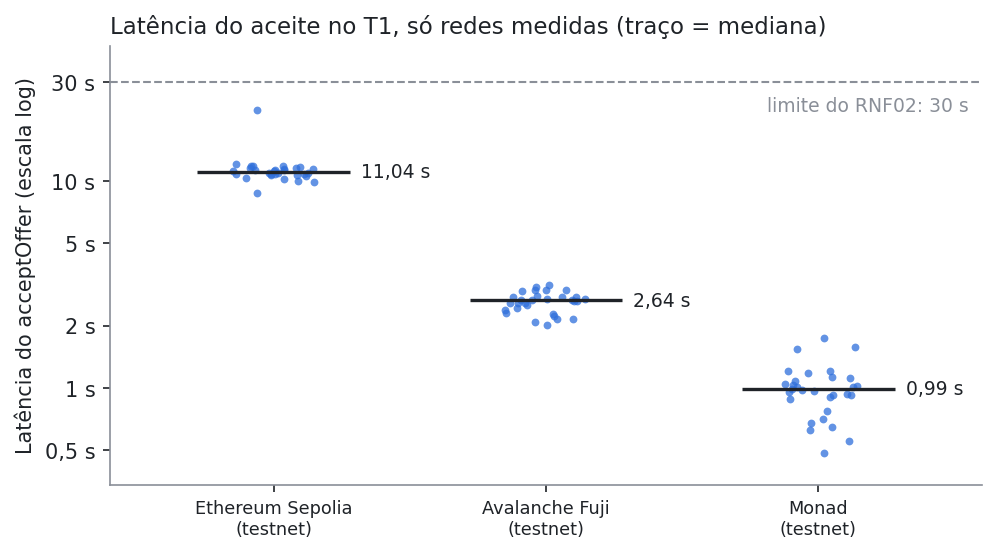
\includegraphics[width=0.85\linewidth]{latencia_t1.png}
\caption{Latência do \fn{acceptOffer} no T1 (30 aceites por rede, escala logarítmica). \pendente{refazer a figura em inglês ou sem título interno, conforme o template}}\label{fig:latencia}
\end{figure}

A Tabela~\ref{tab:notas} traz as notas normalizadas e a pontuação. A Monad ficou em primeiro lugar com 90,1 pontos, seguida pela Avalanche (86,0) e pela Ethereum (58,5). A Figura~\ref{fig:custo} compara o custo do ciclo.

\begin{table}[ht]
\centering
\caption{Notas normalizadas (0 a 1) e pontuação ponderada (0 a 100), cenário base.}\label{tab:notas}
\small
\begin{tabular}{@{}clcccccr@{}}
\toprule
Posição & Rede & C1 & C2 & C3 & C4 & C5 & Pontuação \\
\midrule
1 & Monad & 1,00 & 0,67 & 1,00 & 1,00 & 1,00 & \textbf{90,1} \\
2 & Avalanche & 1,00 & 0,67 & 0,84 & 0,91 & 1,00 & 86,0 \\
3 & Ethereum & 1,00 & 0,67 & 0,00 & 0,00 & 1,00 & 58,5 \\
\bottomrule
\end{tabular}
\end{table}

\begin{figure}[ht]
\centering
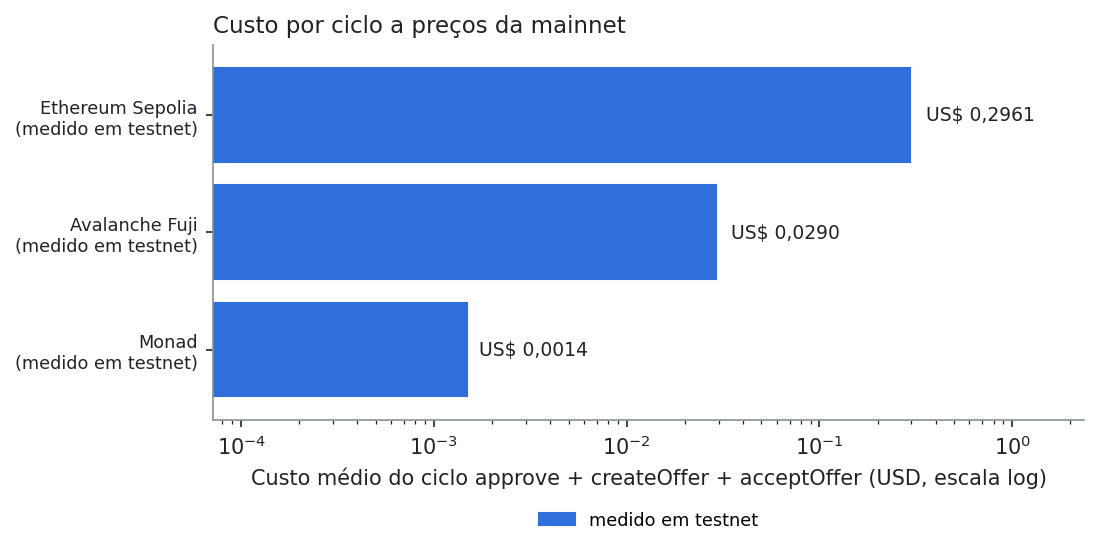
\includegraphics[width=0.85\linewidth]{custo_ciclo.png}
\caption{Custo médio do ciclo a preços da mainnet (escala logarítmica). \pendente{idem}}\label{fig:custo}
\end{figure}

\paragraph{Sensibilidade.} A ordem Monad, Avalanche e Ethereum se manteve nos 17 cenários (base, S1, S2 e S3). A menor pontuação da Monad foi 85,9 (S3 sem C1) e a maior, 100,0 (S3 sem C2); a diferença para a Avalanche variou de 1,8 (S3 sem C3) a 5,8 pontos (S3 sem C1 e S3 sem C2).

\paragraph{Custo de infraestrutura.} Com C4-M2 na pontuação, a ordem passaria a depender da instância da Monad: com servidor físico, Avalanche 85,7, Monad 82,2 e Ethereum 66,4; com instância virtual, Monad 82,2, Avalanche 79,2 e Ethereum 66,4. \pendente{discutir na Seção 5: a recomendação é sensível ao custo de operar um nó da Monad}

\paragraph{Gas da Sepolia após o Glamsterdam.} A Sepolia ativou em 06/10/2026 a atualização Glamsterdam, que encarece a criação de estado \cite{glamsterdam2026}; a mainnet da Ethereum ainda usa as regras anteriores. A Tabela~\ref{tab:glamsterdam} compara o gas do ciclo na Sepolia com o gas na Fuji, que executa o mesmo bytecode com as regras anteriores. O ciclo gastou 3,50 vezes mais na Sepolia. A matriz usa o gas da Sepolia, como define o método; com o gas da Fuji, o custo do ciclo da Ethereum cai de US\$~0,296 para US\$~0,085, a Ethereum continua a mais cara e a ordem não muda (a Avalanche passaria de 86,0 para 82,2 pontos).

\begin{table}[ht]
\centering
\caption{Gas por função: Sepolia (com Glamsterdam) e Fuji (regras anteriores).}\label{tab:glamsterdam}
\small
\begin{tabular}{@{}lrrr@{}}
\toprule
Função & Sepolia & Fuji & Razão \\
\midrule
\fn{approve} & 128.257 & 46.337 & 2,77$\times$ \\
\fn{createOffer} & 927.005 & 220.324 & 4,21$\times$ \\
\fn{acceptOffer} & 446.758 & 163.120 & 2,74$\times$ \\
\fn{cancelOffer} & 133.830 & 51.810 & 2,58$\times$ \\
\midrule
Ciclo completo & 1.502.836 & 429.924 & 3,50$\times$ \\
\bottomrule
\end{tabular}
\end{table}

% -----------------------------------------------------------------------------
\section{Discussão}\label{sec:discussao}

\subsection{Interpretação dos Resultados}

Com três redes EVM públicas executando o mesmo código, três dos cinco critérios não diferenciaram as alternativas: C1 empatou em 100\% de sucesso; C2 teve a mesma nota nas três (mesma linguagem, mesmo código, mesma visibilidade pública); e C5 foi 1,0 em todas, porque o contrato foi implantado sem alteração. O ranking foi decidido por latência e custo, que somam 31,56\% do peso. Como a Monad teve a melhor nota nesses dois critérios e a Ethereum a pior, a ordem se mantém para quaisquer pesos não negativos, o que explica a estabilidade da análise de sensibilidade. \pendente{discutir se o resultado responde à QP ou se, para este conjunto de redes, a decisão se reduz a latência e custo}

A latência de inclusão não conta toda a história. Na Ethereum, a operação só se torna definitiva cerca de 12,8~min após a inclusão \cite{ethereum2024gasper}, o que pesa num produto overnight com janela de liquidação curta; na Avalanche e na Monad a finalidade declarada é inferior a 1~s \cite{avalanche2024consensus,monad2024bft}. Nenhuma das três oferece confidencialidade entre participantes na própria rede: valores, taxas e contrapartes ficam visíveis a qualquer observador, e o sigilo exigido em operações interbancárias teria de ser tratado na aplicação. As três também têm conjunto aberto de validadores, sem governança institucional identificada. \pendente{relacionar com o requisito de sigilo}

O custo absoluto é baixo nas três redes (de US\$~0,0014 a US\$~0,30 por ciclo), mas a diferença relativa é de duas ordens de grandeza. Na Monad, o custo depende do gas limit enviado pelo cliente, e não só do trabalho executado.

Sob carga, a Avalanche apresentou 3 aceites de 64~s no lote de 50 da primeira rodada, acima do limite de 30~s. O horário coincide com uma pausa registrada do observador de blocos do coletor. \pendente{conferir se é efeito da medição antes de citar; a latência do T2 não entra na matriz}

\subsection{Ameaças à Validade e Limitações}\label{sec:ameacas}

\begin{itemize}
\item \textbf{Testnet não é mainnet.} O tráfego é menor, e o custo supõe que o gas da testnet é igual ao da mainnet; para a Ethereum essa premissa deixou de valer durante o estudo (Glamsterdam).
\item \textbf{Uma única janela de coleta.} As três testnets foram coletadas em paralelo, numa janela de 42~min, da mesma máquina e com RPC público; a variação do tráfego ao longo do tempo não foi observada.
\item \textbf{Carga limitada.} Com até 50 aceites simultâneos nenhuma rede falhou; C1 não separou as redes e não mede a capacidade máxima.
\item \textbf{Critérios que empataram.} C1, C2 e C5 deram a mesma nota às três redes; a estrutura de cinco critérios foi pensada para uma lista mais variada.
\item \textbf{Conjunto de redes.} As três redes são públicas, então a confidencialidade não diferenciou as alternativas e a conclusão vale para redes públicas. Incluir ou retirar uma rede muda as notas min-max das demais \cite{belton1983}; por isso a pontuação final foi calculada com a lista já fechada.
\item \textbf{Pesos e escalas.} Os julgamentos do AHP vieram de uma regra por níveis, e não de comparações independentes; as escalas qualitativas (C2-M1, C2-M3, C5) foram definidas pela equipe; as medidas internas de C2 e C4 usam média simples.
\item \textbf{Latência e finalidade.} A latência mede a inclusão no bloco; a janela do requisito de 30~s também inclui backend e interface, e inclusão não é finalidade.
\item \textbf{Dados declarados.} A finalidade e parte das escalas vêm da documentação das próprias redes, não verificada por terceiros \cite{gramoli2023}.
\item \textbf{Generalização.} Um único protocolo foi avaliado; os resultados valem para este caso de uso.
\end{itemize}
\pendente{condensar para caber nas 6 páginas}

% -----------------------------------------------------------------------------
\section{Conclusões e Trabalhos Futuros}\label{sec:conclusao}

Entre as três redes públicas avaliadas, a Monad é a mais adequada para o protocolo de crédito interfinanceiro overnight segundo o modelo de decisão: foi a mais rápida e a mais barata, executou o contrato sem alteração e liderou em todos os cenários de pesos. A Avalanche é uma alternativa próxima, e a Ethereum pública mostrou-se inadequada como camada de liquidação para este caso, pela latência, pelo tempo até a finalidade e pelo custo. O estudo também mostra que testnets podem mudar de regras durante uma coleta, o que exige registrar a versão do protocolo junto com as medições de custo.

Como trabalhos futuros: repetir o T2 com carga maior, até haver falhas; incluir o custo de infraestrutura na pontuação com mais de um provedor; e repetir a coleta em várias janelas. \pendente{revisar}

% -----------------------------------------------------------------------------
\section*{Agradecimentos}
\pendente{omitidos na versão de avaliação}

\section*{Declaração de Uso de IA}
\pendente{obrigatória nas duas versões: descrever quais ferramentas de IA foram usadas, em quais etapas (código de coleta e análise, revisão de texto etc.) e como a equipe verificou o resultado}

\bibliographystyle{unsrt} % trocar pelo estilo numérico ACM do template
\bibliography{referencias}

\end{document}

% =============================================================================
% REFERÊNCIAS DA SEÇÃO 2: ainda não estão em referencias.bib.
% Até serem copiadas para lá, estas citações aparecem sem número no PDF.
% Tudo que vem depois de \end{document} é ignorado pelo LaTeX.
%
% --- NOVAS ---
% @misc{b3taxadi,
%   author = {{B3}},
%   title  = {Taxa {DI}},
%   note   = {Glossário Bora Investir. Acesso em 06/11/2026},
%   url    = {https://borainvestir.b3.com.br/glossario/taxa-di/}
% }
% @article{fishburn1967,
%   author  = {Fishburn, Peter C.},
%   title   = {Letter to the Editor---Additive Utilities with Incomplete Product Sets: Application to Priorities and Assignments},
%   journal = {Operations Research},
%   volume  = {15},
%   number  = {3},
%   pages   = {537--542},
%   year    = {1967},
%   doi     = {10.1287/opre.15.3.537}
% }
% @misc{ethereum2024evm,
%   author = {{Ethereum Foundation}},
%   title  = {Ethereum Virtual Machine ({EVM})},
%   url    = {https://ethereum.org/developers/docs/evm/},
%   note   = {Acesso em 06/11/2026}
% }
% @misc{ethereum2024ssf,
%   author = {{Ethereum Foundation}},
%   title  = {Single Slot Finality},
%   url    = {https://ethereum.org/roadmap/single-slot-finality/},
%   note   = {Acesso em 09/11/2026}
% }
% @misc{ethereum2024networks,
%   author = {{Ethereum Foundation}},
%   title  = {Networks},
%   url    = {https://ethereum.org/developers/docs/networks/},
%   note   = {Acesso em 06/11/2026}
% }
% @misc{iso25010,
%   author = {{ISO/IEC}},
%   title  = {{ISO/IEC} 25010:2023: Systems and Software Engineering --- Systems and Software Quality Requirements and Evaluation ({SQuaRE}) --- Product Quality Model},
%   year   = {2023},
%   note   = {VERIFICAR no catálogo da ISO}
% }
% @article{tolmach2021,
%   author  = {Tolmach, Palina and Li, Yi and Lin, Shang-Wei and Liu, Yang and Li, Zengxiang},
%   title   = {A Survey of Smart Contract Formal Specification and Verification},
%   journal = {ACM Computing Surveys},
%   volume  = {54},
%   number  = {7},
%   year    = {2021},
%   note    = {arXiv:2008.02712. VERIFICAR volume e número no periódico}
% }
% @article{shin2011,
%   author  = {Shin, Yonghee and Meneely, Andrew and Williams, Laurie and Osborne, Jason A.},
%   title   = {Evaluating Complexity, Code Churn, and Developer Activity Metrics as Indicators of Software Vulnerabilities},
%   journal = {IEEE Transactions on Software Engineering},
%   volume  = {37},
%   number  = {6},
%   pages   = {772--787},
%   year    = {2011},
%   doi     = {10.1109/TSE.2010.81}
% }
%
% --- CORRIGIDAS (substituem as entradas de mesma chave) ---
% @misc{bis2020qr,
%   author = {Bech, Morten Linnemann and Hancock, Jenny and Rice, Tara and Wadsworth, Amber},
%   title  = {On the Future of Securities Settlement},
%   year   = {2020},
%   note   = {BIS Quarterly Review, March 2020},
%   url    = {https://www.bis.org/publications/future-securities-settlement}
% }
% @misc{javed2025,
%   author = {Javed, Farhana and Mangues-Bafalluy, Josep},
%   title  = {An Empirical Smart Contracts Latency Analysis on {Ethereum} Blockchain for Trustworthy Inter-Provider Agreements},
%   year   = {2025},
%   note   = {arXiv:2503.01397}
% }
% @misc{lazar2025,
%   author = {Lazăr, Cătălina and Secrieru, Gabriela and Onica, Emanuel},
%   title  = {Where Should {I} Deploy My Contracts? {A} Practical Experience Report},
%   year   = {2025},
%   note   = {arXiv:2504.10535}
% }
% =============================================================================
